\documentclass[preprint,authoryear,review,12pt]{elsarticle}
\usepackage{amsmath}
\usepackage{amsfonts}
\usepackage{lscape}
\usepackage{fullpage}
\usepackage{graphicx,color} % Para escrever em cores
\usepackage{graphics}
\usepackage{subfig}
\usepackage{ae}
\usepackage[T1]{fontenc}
\usepackage[utf8]{inputenc}	
%\usepackage[ansinew]{inputenc}
\usepackage{pdflscape}
\usepackage{url}
\usepackage{setspace}
\usepackage{tabularx}
\usepackage{dcolumn}
\usepackage{rotating}
\usepackage{a4wide}
\usepackage{supertabular}
\usepackage[lmargin=1.5cm, rmargin=1.5cm,tmargin=1.50cm,bmargin=1.50cm]{geometry}
\usepackage{fullpage}
\usepackage{multirow}
\usepackage{longtable}
\usepackage{geometry}
\usepackage[all]{xy}
\usepackage{lscape}
\usepackage{pdflscape}
\usepackage{tabularx}
\usepackage{tabulary}
\usepackage{textgreek}
\usepackage{fixmath}
\usepackage{longtable}
\usepackage{subfig}
\usepackage{graphicx}

\usepackage{booktabs}         % Recommended for professional cell borders
\usepackage[flushleft]{threeparttable}% [flushleft] left-aligns the footnotes
\usepackage{threeparttablex}
\usepackage{longtable}

\usepackage{nicematrix}
\usepackage{enumitem}

%
\usepackage[table,xcdraw]{xcolor}
\usepackage{lipsum}
%\usepackage[margin=1in]{geometry} 
\usepackage{mathtools}
\usepackage{upgreek}
\usepackage{booktabs,caption} %
\usepackage[flushleft]{threeparttable} % Rodapé
\usepackage{float} % Fixar local tabela [H]
\usepackage{arydshln} 
\usepackage[normalem]{ulem}
 \useunder{\uline}{\ul}{}
%
\usepackage{calrsfs}
\definecolor{mygray}{gray}{0.6}
\definecolor{myblue}{RGB}{30 0, 180}

% The amssymb package provides various useful mathematical symbols
\usepackage{mathtools, amsmath, amssymb, amsthm, latexsym}

%\usepackage[top=2cm, left=2cm, right=2cm, bottom=2cm]{geometry}
\usepackage{rotating}

\newcommand{\m}[3]{\multicolumn{#1}{#2}{#3}}
\newcolumntype{d}[1]{D{.}{.}{#1}}

\def\mathbi#1{\textbf{\em #1}}
\newcommand{\mat}[1]{\mbox{\boldmath{$#1$}}}

%%% Nota: abrir com Western (ISO Latin 1) %%%%%
\usepackage{hyperref} % para as citaes e refs voltarem a cor normal comentar esta parte
\hypersetup{
  colorlinks = true,
  linkcolor=blue,   % color of internal links
  citecolor=blue,   % color of links to bibliography
  urlcolor=blue,    % color of external links
  pagebackref=true,
  implicit=false,
  bookmarks=true,
  bookmarksopen=true,
  pdfdisplaydoctitle=true
} 

%\usepackage{dcolumn}

%\journal{Empirical Economics}
\makeatletter
\def\ps@pprintTitle{%
 \let\@oddhead\@empty
 \let\@evenhead\@empty
 \def\@oddfoot{}%
 \let\@evenfoot\@oddfoot}
\makeatother

\begin{document}

\begin{frontmatter}
\title{Uncovered Interest Parity, Inverted: Risk-Premium Transmission of Monetary Policy Shocks in Brazil}

% Uncovered Interest Parity, Inverted: Risk-Premium Transmission of Monetary Policy Shocks in Brazil
% Beyond Uncovered Interest Parity: Risk-Premium Transmission of Monetary Policy Shocks in Brazil


\author[Label0]{Gabriel Arruda}
\author[Label1]{Jo\~ao F. Caldeira }
%\author[Label1]{Guilherme V. Moura}
\address[Label0]{Graduate School of Economics\\Universidade Federal de Santa Catarina}
\address[Label1]{Department of Economics\\Universidade de Brasília \& CNPq}

\begin{abstract}
Ao contrário do que prevê o mecanismo tradicional da paridade descoberta da taxa de juros, um choque contracionista de 50 pontos-base na política monetária brasileira deprecia a moeda doméstica e, simultaneamente, eleva o prêmio de risco soberano. Após o choque, a taxa de câmbio BRL/USD deprecia $3,\!64\%$ no impacto, enquanto o EMBI+ e o CDS soberano de cinco anos apresentam elevação significativa, uma resposta conjunta consistente com um canal de transmissão via prêmio de risco, no qual o aumento da percepção de risco soberano domina o efeito convencional do diferencial de juros. A curva de juros reforça essa evidência: a resposta das taxas cresce sistematicamente com a maturidade até cinco anos, exibindo amplificação superior à documentada em estudos comparáveis para economias desenvolvidas. No médio prazo, a taxa de câmbio, as medidas de risco soberano e a curva de juros apresentam dinâmica de reversão altamente sincronizada, oferecendo evidência adicional de um mecanismo comum de transmissão. Esses resultados contrastam com evidências recentes obtidas por meio de identificação por heterocedasticidade em frequência diária, que rejeitam a hipótese de dominância fiscal para o Brasil, sugerindo que a importância do canal de prêmio de risco pode depender da frequência dos dados e da estratégia de identificação adotada. Os resultados são obtidos a partir de um Modelo de Fatores Dinâmicos Estruturais (SDFM) identificado por instrumento externo, combinando surpresas monetárias em reuniões do Copom, ortogonalização em relação à informação pública predeterminada e um filtro de sinal que separa choques de política monetária de choques de informação do Banco Central, utilizando um painel com 106 séries macroeconômicas e financeiras brasileiras entre 2013 e 2025.\\

\noindent Abstract: Contrary to the conventional prediction of Uncovered Interest Parity (UIP), a 50-basis-point contractionary monetary policy shock in Brazil depreciates the domestic currency while simultaneously increasing sovereign risk premia. Rather than attracting capital through a wider interest-rate differential, tighter monetary policy is followed by a $3.64\%$ on-impact depreciation of the BRL/USD exchange rate, accompanied by significant increases in both the EMBI+ and the five-year sovereign CDS spread. This joint response points to a risk-premium transmission channel in which the deterioration of sovereign risk dominates the standard interest-rate channel. The yield curve reinforces this interpretation: the response of interest rates increases systematically with maturity up to five years, exhibiting stronger amplification than that documented for comparable studies of advanced economies. Over the medium run, the exchange rate, sovereign risk measures, and the yield curve display highly synchronized reversal dynamics, providing additional evidence of a common transmission mechanism. These findings differ from recent evidence based on daily heteroskedasticity identification, which rejects the fiscal dominance hypothesis for Brazil, suggesting instead that the importance of the risk-premium channel may depend on both the data frequency and the identification strategy employed. Our results are obtained from a Structural Dynamic Factor Model (SDFM) identified through an external instrument, combining monetary policy surprises around Copom meetings, orthogonalization with respect to predetermined public information, and a sign-restriction filter that separates monetary policy shocks from central bank information shocks, using a panel of more than one hundred Brazilian macroeconomic and financial time series spanning 2013–2025.

\end{abstract}



\begin{keyword}
Structural Factor Models  \sep Monetary Policy  \sep Asset Prices \sep Sovereign Risk \sep External Instruments
\\[0.1in]
JEL C32 \sep E52 \sep E43 \\[0.1in]
\end{keyword}


\end{frontmatter}
%\newpage
 %\singlespacing  
\onehalfspacing   
% \doublespacing  
%
% henceforth DNS
\section{Introduction}
A compreensão dos canais de transmissão da política monetária constitui um dos temas centrais da macroeconomia, uma vez que as decisões do banco central afetam diretamente as condições de crédito, as expectativas dos agentes e a atividade econômica. Entre esses canais, o canal cambial ocupa posição de destaque. Segundo o mecanismo convencional da paridade descoberta da taxa de juros, um aperto monetário amplia o diferencial de juros doméstico, atrai capital estrangeiro e aprecia a moeda doméstica. Essa previsão, entretanto, pressupõe que o diferencial de juros seja a principal margem de ajuste dos fluxos internacionais de capitais, hipótese que pode deixar de ser válida quando preocupações com a sustentabilidade fiscal passam a desempenhar papel relevante na precificação dos ativos. Esse tipo de reversão da previsão convencional da paridade descoberta não é exclusivo de contextos de dominância fiscal: \cite{dalgicozhan2026} mostram, em um arcabouço teórico e empírico para economias emergentes, que a interação entre descasamento cambial de passivos bancários e faturamento de exportações em dólar (dominant currency pricing) também é capaz de gerar prêmios de risco cambial endógenos que dominam o canal convencional do diferencial de juros, fazendo com que depreciações ocorram justamente nos estados em que os ativos domésticos deveriam, pela UIP padrão, se valorizar.

%A compreensão dos canais de transmissão da política monetária é um dos temas centrais da macroeconomia, pois as decisões do banco central afetam diretamente as condições de crédito, as expectativas dos agentes e a atividade econômica. Entre os canais de transmissão, a resposta da taxa de câmbio ocupa um lugar particular: segundo o mecanismo convencional da paridade descoberta da taxa de juros, um aperto monetário deveria atrair capital estrangeiro e apreciar a moeda doméstica. Esse mecanismo, no entanto, pressupõe que o diferencial de juros seja a única margem relevante de ajuste, uma suposição que pode falhar em economias cuja trajetória fiscal é vista pelos mercados como uma restrição ativa.

Neste artigo, documentamos um fato estilizado que contraria essa previsão: em uma economia emergente sujeita a preocupações fiscais, um choque contracionista de política monetária pode elevar o prêmio de risco soberano a ponto de inverter a resposta convencional da taxa de câmbio. Utilizando dados brasileiros entre 2013 e 2025, encontramos que um aperto monetário de 50 pontos-base deprecia o real e, simultaneamente, eleva o EMBI+ e o CDS soberano de cinco anos. Essa resposta conjunta é difícil de reconciliar com o canal tradicional da paridade descoberta da taxa de juros, mas é consistente com um mecanismo de transmissão via prêmio de risco, no qual esse efeito domina o impacto convencional do diferencial de juros. A curva de juros reforça essa interpretação: o repasse do choque cresce sistematicamente com a maturidade até cinco anos, superando a amplificação documentada em estudos comparáveis para economias desenvolvidas, e reverte no médio prazo em estreita sincronia com a taxa de câmbio e as medidas de risco soberano. Em conjunto, essas evidências são compatíveis com um ambiente de dominância fiscal, no qual elevações da taxa básica de juros intensificam as preocupações quanto à sustentabilidade da dívida pública e elevam o prêmio de risco soberano, embora o objetivo deste artigo não seja testar diretamente essa hipótese.

%Neste artigo, documentamos um fato estilizado que contraria essa previsão: em determinadas economias emergentes, um choque contracionista de política monetária pode elevar o prêmio de risco soberano a ponto de inverter a resposta esperada da taxa de câmbio. Usando dados brasileiros entre 2013 e 2025, mostramos que um aperto monetário de 50 pontos-base deprecia o real e, simultaneamente, eleva o EMBI+ e o CDS soberano de cinco anos, uma resposta conjunta incompatível com o canal tradicional da paridade de juros, mas consistente com um regime em que o aumento da taxa de juros piora a percepção sobre a sustentabilidade da dívida e esse efeito domina o diferencial de juros convencional. A curva de juros reforça essa leitura: o repasse do choque cresce com a maturidade até cinco anos, superando a amplificação documentada em desenhos comparáveis para economias desenvolvidas, e reverte no médio prazo em sincronia com o câmbio e o prêmio de risco soberano.

Até onde sabemos, este é o primeiro trabalho a documentar esse mecanismo de transmissão para a economia brasileira utilizando um Modelo de Fatores Dinâmicos Estruturais identificado por instrumento externo. Ao relacionar conjuntamente a resposta da taxa de câmbio, do prêmio de risco soberano e da curva de juros, o artigo fornece evidência de que o canal de prêmio de risco pode desempenhar papel relevante na transmissão da política monetária em economias emergentes com fragilidades fiscais como a brasileira.

Identificar empiricamente esse mecanismo de transmissão, entretanto, não é uma tarefa trivial. Choques de política monetária não são diretamente observáveis e sua identificação depende da informação disponível ao econometrista. Modelos tradicionais, como os Vetores Autorregressivos Estruturais (SVAR), frequentemente sofrem do problema da não-fundamentalidade, uma vez que operam com conjuntos de informação muito menores do que aqueles observados pelos agentes econômicos e pelo próprio banco central. Como consequência, podem subestimar a magnitude dos choques monetários ou produzir respostas aparentemente contraintuitivas para algumas variáveis macroeconômicas e financeiras \citep[]{villaverde, alessi}. Para contornar essa limitação, empregamos um Modelo de Fatores Dinâmicos Estruturais (SDFM), que extrai fatores comuns de um amplo conjunto de variáveis macroeconômicas e financeiras, aproximando o conjunto de informação relevante utilizado pelos agentes econômicos e permitindo uma identificação mais robusta dos choques monetários \citep[]{STOCK2016415, alessi}.

%A identificação correta desse mecanismo depende crucialmente da informação disponível para o econometrista. Modelos tradicionais, como os Vetores Autorregressivos Estruturais (SVAR), frequentemente sofrem do problema da não-fundamentalidade, pois não conseguem incorporar o vasto conjunto de dados que os agentes econômicos e o próprio banco central utilizam em suas decisões, o que pode levar a uma má especificação do choque monetário \citep[]{villaverde}. Como consequência, os SVARs tendem a subestimar a magnitude do impacto da política monetária e a gerar respostas contraintuitivas em algumas variáveis \citep[]{alessi}. Para superar essa limitação, este estudo emprega um Modelo de Fatores Dinâmicos Estruturais (SDFM), que extrai fatores comuns de um amplo conjunto de variáveis macroeconômicas e financeiras, aproximando o espaço de informação relevante e permitindo uma identificação mais robusta dos choques \citep[]{STOCK2016415, alessi}.

A identificação do choque monetário é realizada por meio de um instrumento externo construído a partir das surpresas de juros observadas em dias de reunião do Copom, combinando a ortogonalização por informação predeterminada de \cite{bauer2023} e a regra de sinal de \cite{jarocinski2020}, que separa choques de política de choques de informação do banco central. A relevância do instrumento é avaliada pela estatística de Wald de \cite{montielolea}, complementar ao F robusto de primeiro estágio.

O modelo é estimado utilizando um painel com 106 séries macroeconômicas e financeiras brasileiras, abrangendo atividade econômica, mercado de trabalho, inflação, crédito, agregados monetários e preços de ativos entre janeiro de 2013 e setembro de 2025. Esse amplo conjunto de informações permite identificar os choques monetários de forma mais robusta do que em VARs de pequena dimensão e acompanhar sua transmissão simultânea para diversas classes de ativos, câmbio, prêmio de risco soberano, curva de juros, crédito e mercado acionário, dimensão conjunta que desenhos de menor escala não permitem capturar.

Nossos resultados também diferem das evidências recentes para o Brasil obtidas por identificação via heterocedasticidade em frequência diária, que rejeitam a hipótese de dominância fiscal \cite{goncalves2025}. Essa divergência sugere que a importância do canal de prêmio de risco pode depender da frequência dos dados e da estratégia de identificação utilizada, uma questão que discutimos ao longo do artigo.

O restante deste artigo está organizado da seguinte forma. A Seção 2 revisa a literatura sobre identificação de choques monetários e canais de transmissão para preços de ativos. A Seção 3 descreve o modelo de fatores dinâmicos estruturais, a base de dados e a estratégia de identificação por instrumento externo. A Seção 4 apresenta os resultados, com ênfase no canal de câmbio e risco soberano. A Seção 5 conclui.

%A compreensão dos canais de transmissão da política monetária é um dos temas centrais da macroeconomia, pois as decisões do banco central afetam diretamente as condições de crédito, as expectativas dos agentes e a atividade econômica. Dentre os diversos canais, a resposta dos preços dos ativos financeiros — como ações, títulos e a taxa de câmbio — é particularmente relevante, pois reflete a reação imediata dos mercados e serve como um importante mecanismo de transmissão para a economia real. A literatura recente tem dedicado atenção considerável a quantificar essa relação, utilizando modelos cada vez mais sofisticados para isolar o impacto de choques monetários na precificação de risco (e.g., \cite{BEKAERT2013771}, \cite{alessi}). No contexto de economias emergentes como o Brasil, caracterizadas por maior volatilidade e particularidades institucionais, a análise desses efeitos torna-se ainda mais crucial para a condução da política monetária e a gestão de portfólios.

%A correta identificação desses efeitos depende crucialmente da informação disponível para o econometrista. Modelos tradicionais, como os Vetores Autorregressivos Estruturais (SVAR), frequentemente sofrem do problema da não-fundamentalidade, pois não conseguem incorporar o vasto conjunto de dados que os agentes econômicos e o próprio banco central utilizam em suas decisões, o que pode levar a uma má especificação do choque monetário \cite{villaverde}. Estudos mostram que, por consequência, os SVARs tendem a subestimar a magnitude do impacto da política monetária e a gerar respostas contraintuitivas em algumas variáveis \cite{alessi}.

%Para superar essa limitação, este estudo emprega um Modelo de Fatores Dinâmicos Estruturais (SDFM). Ao extrair fatores comuns de um grande conjunto de variáveis macroeconômicas e financeiras, o SDFM permite uma identificação mais robusta dos choques, capturando a informação relevante de maneira parcimoniosa \cite{STOCK2016415}. A principal contribuição deste trabalho é, portanto, fornecer uma quantificação mais precisa dos canais de transmissão da política monetária no Brasil, mostrando que os efeitos sobre os preços dos ativos são mais fortes e rápidos do que a literatura baseada em modelos de menor dimensão tipicamente encontra. O restante do artigo detalha a metodologia, os dados e aprofunda a análise dos resultados.

%O desenho é o de \cite{alessi}, aplicado a uma economia emergente com regime de dívida distinto do europeu e do americano. O instrumento é construído sobre surpresas de DI em dias de reunião do Copom. Ele combina a ortogonalização por informação predeterminada de \cite{bauer2023} e a regra de sinal de \cite{jarocinski2020}. A relevância é avaliada pela estatística de \cite{montielolea} e não pela F de primeiro estágio.

\section{Revisão de literatura}

Dois problemas separam as estimativas do efeito da política monetária sobre preços de ativos. O primeiro é o tamanho do conjunto de informação do modelo. O segundo é a identificação do choque. A literatura tratou os dois em linhas quase independentes.

Um VAR de pequena dimensão raramente contém a informação que o banco central observa. \cite{villaverde} formalizam a condição sob a qual as inovações de um VAR geram o mesmo espaço que os choques estruturais. Ela falha em modelos de equilíbrio geral usuais. Quando falha, a reação sistemática do banco central a informação omitida aparece como choque de política.

A resposta da literatura foi ampliar o painel. \cite{bernanke} extraem fatores de um conjunto amplo de séries e os incluem no VAR, o modelo FAVAR. \cite{STOCK2016415} tratam o caso geral, em que o modelo de fatores dinâmicos substitui o VAR e a identificação opera sobre as inovações fatoriais. Trabalhos posteriores aplicam a mesma lógica à transmissão global da política americana \cite{miranda} e ao sentimento do investidor \cite{lutz}.

O argumento tem uma pré-história empírica. \cite{bagliano1998} confrontam os choques de um VAR monetário com medidas de surpresa extraídas de mercados futuros. Essas medidas usam o conjunto de informação de que os mercados dispõem, ao contrário da função de reação estimada. Ainda assim produzem funções de resposta que não diferem estatisticamente das do VAR de referência.

\cite{alessi} isolam o efeito do conjunto de informação mantendo a identificação fixa. Os autores estimam um VAR de quatro variáveis e um modelo de fatores dinâmicos de grande escala sobre os mesmos dados. O instrumento de alta frequência, a ordem de defasagens e a normalização de 50 pontos-base no yield soberano de 2 anos são os mesmos nos dois modelos. Os painéis reúnem 88 séries para a área do euro e 95 para os Estados Unidos.

As diferenças entre os dois modelos são grandes. Nos dados americanos, a resposta do prêmio excedente dos títulos corporativos no impacto é o dobro no modelo de fatores. Os preços de imóveis caem cerca de 1,5\% em dois anos no modelo de fatores e sobem no VAR. A maioria das especificações do VAR produz aumento da produção industrial após um aperto. Como apenas o conjunto de informação varia, a diferença não pode ser atribuída à hipótese de identificação.

Os modelos teóricos que motivam essa literatura tratam o preço dos ativos como canal de transmissão. \cite{castelnuovo} incorporam rigidez nominal de salários e heterogeneidade de investidores em um modelo DSGE, e obtêm efeito da riqueza financeira sobre o consumo. \cite{Cooley} mostram, em equilíbrio geral com firmas heterogêneas, que a estrutura financeira da firma condiciona sua resposta ao choque monetário. As previsões que o trabalho empírico procura medir são a reprecificação imediata e a resposta desigual entre classes de ativos.

A identificação por instrumento externo trata o segundo problema sem impor restrições de exclusão sobre a matriz de impacto. \cite{mertensravn2013} são a referência de origem do estimador para o caso geral com múltiplos instrumentos. Os autores tratam as séries narrativas de mudanças tributárias não como observações do choque, mas como variáveis correlacionadas com ele. Registros históricos raramente são inequívocos. Uma série tratada como o próprio choque produz estimativas atenuadas pelo erro de medida, e o mesmo erro não compromete sua validade como instrumento.

As condições que enunciam são relevância, $E[m_t \varepsilon_{1t}'] = \Phi$ não singular, e exogeneidade, $E[m_t \varepsilon_{2t}'] = 0$, sobre os demais choques estruturais. Os autores também medem a qualidade da proxy. As confiabilidades estimadas de suas duas séries narrativas são $0{,}30$ e $0{,}69$, o que corresponde a correlações de $0{,}55$ e $0{,}83$ com os choques latentes. A leitura que fazem é que o erro de medida em séries narrativas é grande na prática.

\cite{stockwatson2018} separam o que cada estimador exige. O SVAR-IV projeta o instrumento sobre as inovações do VAR e propaga a resposta pela dinâmica estimada. Exige relevância, exogeneidade contemporânea e invertibilidade, esta última a hipótese de que os choques estruturais podem ser recuperados de valores correntes e passados das observáveis.

O LP-IV estima uma regressão de variável instrumental por horizonte e dispensa a invertibilidade. Em troca, exige exogeneidade também em relação a choques passados e futuros. A parte restritiva é a que envolve choques passados.

A saída fácil desse dilema não existe. Incluir defasagens genéricas das observáveis como controles, para salvar um instrumento correlacionado com choques passados, equivale a supor invertibilidade. Nesse caso o SVAR-IV é o estimador mais eficiente. Os mesmos autores apontam o modelo de fatores como caminho para a invertibilidade, com a ressalva de que ampliar o número de variáveis não a garante.

\cite{gertler2015} levam o instrumento externo para a política monetária. A surpresa é medida sobre contratos futuros de juros, em janela de 30 minutos em torno dos anúncios do Federal Open Market Committee. Os autores separam instrumento de política, a taxa overnight, de indicador de política, uma taxa de prazo mais longo cuja inovação mensal incorpora a revisão das expectativas de juros.

A escolha do indicador é empírica. Os autores adotam a taxa de 1 ano, e não a de 2 anos que preferem conceitualmente. A razão é que nenhuma combinação de surpresas alcança primeiro estágio utilizável para a taxa de 2 anos. A F de primeiro estágio da taxa de 1 ano é $21{,}5$, contra o limiar convencional de 10. O resultado substantivo é que uma alta de 20 pontos-base nessa taxa eleva as taxas de crédito corporativo em cerca de 15 pontos-base. Quase todo o aumento vem de prêmio de prazo e spread de crédito.

Duas críticas posteriores mostram que a surpresa bruta não satisfaz a exogeneidade. \cite{jarocinski2020} observam que cerca de um terço dos anúncios do Federal Open Market Committee desde 1990 traz juros e ações subindo juntos. O co-movimento é incompatível com um choque de política pura. Os autores atribuem esses dias a um choque de informação do banco central. A separação usa o sinal do co-movimento e zera a surpresa nos dias de sinal positivo. Com ela, a resposta dos juros fica menos persistente e a queda do nível de preços mais pronunciada, o que atenua o \textit{price puzzle}.

\cite{bauer2023} chegam ao mesmo sintoma por outra via. Os autores mostram que a surpresa de alta frequência é previsível por notícias públicas anteriores ao anúncio, com $R^2$ entre $0{,}12$ e $0{,}20$. A causa que apontam é que o mercado subestima a resposta do Federal Reserve às notícias. Nenhuma informação privada do banco central é necessária para gerar o padrão.

O remédio é regredir a surpresa sobre essa informação predeterminada e usar o resíduo como instrumento. A correção vale para identificação em VAR e em \textit{local projections}, e é dispensável em estudos de evento com preços de ativos. As duas camadas atacam problemas distintos, contaminação por informação e previsibilidade, e podem ser aplicadas em conjunto, embora a literatura não tenha formalizado essa combinação..

\cite{montielolea} tratam a inferência quando o instrumento é fraco. A função de resposta identificada por instrumento externo é uma razão entre quantidades assintoticamente normais, e o denominador dessa razão é a própria relevância. Quando ela é pequena, o estimador de plug-in é inconsistente e viesado na direção da resposta que a decomposição de Cholesky produziria com o choque ordenado em primeiro lugar. A consequência prática é direta. A proximidade entre uma estimativa recursiva e uma por instrumento externo não corrobora a ordenação recursiva, a menos que a força do instrumento seja verificada.

Paralelamente à discussão sobre identificação, uma literatura recente documenta que a resposta cambial a choques de juros pode se afastar da previsão convencional da paridade descoberta quando fragilidades estruturais tornam o prêmio de risco endógeno ao próprio choque. \cite{dalgicozhan2026}, por exemplo, mostram que em economias com descasamento cambial nos balanços bancários e faturamento de exportações em dólar, um aperto monetário externo eleva o prêmio de risco cambial exigido pelos investidores, atenuando ou revertendo a apreciação que a paridade descoberta prescreveria. Embora a fonte de fragilidade nesse caso seja financeiro-cambial, e não fiscal, o resultado ilustra que a dominância do canal de prêmio de risco sobre o diferencial de juros não é uma singularidade brasileira, mas um fenômeno documentado em diferentes contextos institucionais. Se um mecanismo análogo opera no Brasil por meio do canal fiscal, contudo, é uma questão que a literatura recente ainda não resolve.

Para o Brasil, \cite{goncalves2025} identificam choques monetários por heterocedasticidade, no desenho de \cite{rigobon2003}. A comparação é entre semanas com e sem reunião do Copom. Os autores usam variações diárias de quarta para quinta-feira, em 768 observações entre 2009 e 2024. As surpresas vêm de contratos de DI em quatro vencimentos, e as expectativas de inflação de títulos indexados.

Um aperto de 100 pontos-base reduz a expectativa de inflação de 1 ano entre $0{,}20$ e $0{,}27$ ponto percentual, e a de 5 anos entre $0{,}53$ e $0{,}69$ ponto percentual. O real aprecia entre $3{,}4\%$ e $5{,}6\%$, e o CDS de 5 anos não responde. A leitura dos autores é que a política monetária ancora expectativas mesmo com dívida elevada, o que rejeita a hipótese de dominância fiscal em frequência diária. As estimativas mensais deste trabalho divergem no sinal do câmbio e na resposta do risco soberano, desacordo retomado na seção de resultados.


\section{Metodologia e Estratégia Empírica}
\label{sec:metodologia}

\subsection{O Modelo de Fatores Dinâmicos Estruturais}

O modelo empírico é um Modelo de Fatores Dinâmicos Estruturais (SDFM), representado por três equações:
\begin{align}
    \overset{n\times 1}{X_t} &= \overset{n\times r}{\Lambda} \overset{r\times 1}{F_t} + \overset{n\times 1}{e_t}\label{eq:4}\\[4pt]
    \overset{r\times r}{\Phi(L)}\overset{r\times 1}{F_t} &= \overset{r\times q}{G} \overset{q\times 1}{\eta_t} \label{eq:5}\\[4pt]
    \overset{q\times 1}{\eta_t} &= \overset{q\times q}{H} \overset{q\times 1}{\varepsilon_t} \label{eq:6}
\end{align}
A \ref{eq:4} é a equação de observação: o vetor de $n$ variáveis observáveis $X_t$ decompõe-se em um componente comum, dado por $r$ fatores latentes $F_t$ e pela matriz de cargas $\Lambda$, e um componente idiossincrático $e_t$. A \ref{eq:5} descreve a dinâmica dos fatores, com $\Phi(L) = I - \Phi_1 L - \dots - \Phi_p L^p$ um polinômio de defasagens de ordem $p$ e $\eta_t$ um vetor de $q$ inovações fatoriais. A \ref{eq:6} liga essas inovações aos $q$ choques estruturais $\varepsilon_t$ pela matriz $H$. A ordem do VAR dos fatores é fixada em $p = 6$, suficiente para acomodar a persistência das séries mensais brasileiras sem sobreparametrizar a dinâmica.

Combinando as três equações, o modelo assume a forma de média móvel que escreve as observáveis em termos dos choques estruturais:
\begin{align}\label{eq:7}
    X_t=\Lambda \Phi(L)^{-1}GH\varepsilon_t + e_t
\end{align}
A estimação requer determinar o número de fatores estáticos $r$ e dinâmicos $q$ e normalizar as matrizes $\Lambda$, $G$ e $H$.

O conjunto de séries é não-estacionário por construção, pois reúne séries em nível, séries em taxa e séries já diferenciadas, com ordens de integração distintas. Extrair fatores diretamente sobre esse conjunto faria com que as séries de maior variância dominassem a decomposição. Seguindo \cite{barigozzi2016non}, cada série sem tendência $X_{it}$ é dividida pelo desvio padrão de sua primeira diferença $s_{iy}$:
\begin{equation}
    Z_{it} = \frac{X_{it}}{s_{iy}}
\end{equation}
A padronização equaliza a escala das flutuações sem diferenciar as séries, o que preserva a informação de baixa frequência usada pelo modelo. Por essa razão os critérios de \cite{bai-ng} não entram na forma padrão: eles pressupõem séries estacionárias. O tratamento de \cite{barigozzi2016non} mantém a estrutura de fatores válida sob não-estacionariedade.

O uso de um grande conjunto de séries responde ao problema de não-fundamentalidade dos choques estruturais \cite{villaverde}. Um VAR de pequena dimensão raramente contém a informação que os agentes e o banco central de fato observam, e o choque recuperado nesse espaço restrito é uma combinação de choques estruturais, não o choque de política monetária isolado. Ao extrair fatores comuns de um conjunto amplo de variáveis, o SDFM aproxima o espaço de informação relevante e recupera choques fundamentais, como mostram \cite{alessi} ao comparar o SDFM a um VAR de referência sob o mesmo instrumento.

\subsection{Base de Dados}

A base reúne cerca de 110 séries mensais para a economia brasileira entre janeiro de 2013 e setembro de 2025, o que corresponde a 147 meses após o alinhamento das séries. O início em 2013 acompanha a mudança metodológica da PNAD Contínua no mercado de trabalho. As fontes são oficiais (Banco Central do Brasil, IBGE, B3, Tesouro Nacional e ANBIMA), somadas a indicadores de risco soberano e mercado externo (EMBI, CDS de cinco anos e MSCI) e a um índice de incerteza de política econômica (EPU). Os blocos cobrem atividade real, mercado de trabalho, inflação, commodities, agregados monetários e de crédito, e preços de ativos.

As taxas de juros de maturidade fixa (3 meses, 6 meses, 1, 2, 5 e 10 anos) vêm do ajuste do modelo de \cite{svensson1994estimating} sobre os contratos de DI futuro em cada data. As séries nominais entram em logaritmo e, quando os testes indicam componente sazonal, são ajustadas pelo procedimento X-13ARIMA-SEATS \cite{sax2018seasonal}. A lista completa de séries, fontes e transformações está no Anexo \ref{anexo-A} (\autoref{tab:lista_variaveis}).

\subsection{Identificação por instrumento externo}

A identificação do choque de política monetária usa um instrumento externo, no arcabouço de proxy-SVAR de \cite{stockwatson2018} e \cite{gertler2015}, transposto para o DFM como em \cite{alessi}. A abordagem dispensa a ordenação recursiva entre os fatores. No lugar dela entra uma variável observada fora do modelo, correlacionada com o choque de interesse e ortogonal aos demais choques estruturais.

Seja $z_t$ o instrumento e $\varepsilon_t^{p}$ o choque de política monetária. O instrumento é válido sob duas condições: relevância, $E[z_t \varepsilon_t^{p}] \neq 0$, e exogeneidade, $E[z_t \varepsilon_t^{j}] = 0$ para todo choque estrutural $j \neq p$ \cite{stockwatson2018}. Sob essas condições, a projeção das inovações fatoriais $\eta_t$ sobre o instrumento identifica, a menos de escala, a coluna de $H$ associada ao choque de política monetária. Empilhando $\eta_t$ e $z_t$ na amostra alinhada, essa coluna é estimada por $\hat{H}_{\cdot p} = (Z'\eta)/(Z'Z)$. O alinhamento temporal segue a implementação computacional de \cite{alessi}.

O choque é normalizado para elevar o yield de 6 meses em 50 pontos-base no impacto, ou $0{,}005$ em proporção decimal. A escolha do yield de 6 meses como variável de política, em vez da Selic overnight, segue a distinção de \cite{gertler2015} entre o instrumento de política, a taxa overnight, e o indicador de política, uma taxa de prazo mais longo que incorpora a revisão das expectativas de juros embutida na decisão. No caso brasileiro a distinção é mais aguda. As decisões do Copom saem após o fechamento do mercado, e a surpresa é medida na curva de DI entre a quarta e a quinta-feira, não na taxa overnight. A Selic mensal, uma média do overnight dentro do mês, quase não embute essa surpresa. Sob o diagnóstico de relevância de \cite{montielolea}, a normalização pela Selic não alcança o limiar de instrumento utilizável em nenhuma dimensão da varredura de especificações, enquanto a normalização pelo yield de 6 meses alcança, como reporta a \autoref{tab:rq_sweep}.

\subsection{Construção do instrumento}

O instrumento primário combina três camadas: a surpresa de juros em dias de reunião do Copom, medida como em \cite{gertler2015}, a ortogonalização em relação à informação pública anterior ao anúncio, de \cite{bauer2023}, e o filtro de sinal de \cite{jarocinski2020}, que separa choques de política de choques de informação.

A primeira camada mede a surpresa como a variação do DI futuro no vértice de 126 dias úteis, cerca de 6 meses, entre o fechamento da quarta-feira da reunião e o da quinta-feira seguinte. A decisão do Copom é anunciada após o fechamento do mercado, de modo que a janela de um dia captura a primeira sessão em que os preços incorporam a decisão. A amostra tem 95 reuniões entre 2013 e 2025. As surpresas são somadas dentro de cada mês, o esquema de agregação de \cite{jarocinski2020}, e o instrumento vale zero nos meses sem reunião.

A segunda camada remove o componente previsível da surpresa. \cite{bauer2023} mostram que surpresas de alta frequência são correlacionadas com informação pública anterior ao anúncio, porque o mercado subestima a resposta do banco central às notícias. Uma surpresa previsível viola a exogeneidade do instrumento. Seguindo o desenho dos autores, a surpresa é regredida sobre preditores medidos até o fechamento da quarta-feira: uma tendência temporal, as variações acumuladas em 65 pregões do Ibovespa, do S\&P 500, do VIX, do petróleo Brent, do câmbio BRL/USD e da inclinação da curva de DI (2 anos menos 3 meses), e as revisões em 20 pregões das medianas da pesquisa Focus para o IPCA acumulado em 12 meses e para a Selic no fim do ano seguinte. A inclusão do retorno do Ibovespa entre os preditores também tem motivo de identificação, porque a regra de política estimada por \cite{castelnuovo} responde a condições do mercado acionário, canal que a ortogonalização precisa remover da surpresa antes do filtro de sinal. O resíduo dessa regressão é a surpresa ortogonalizada. O $R^2$ é $0{,}024$, na faixa esperada. \cite{bauer2023} obtêm entre $0{,}12$ e $0{,}20$ incluindo surpresas de divulgações macroeconômicas que não existem em frequência diária para o Brasil, e um $R^2$ alto indicaria vazamento de informação contemporânea na regressão. A exigência de que todos os preditores sejam predeterminados disciplina a especificação. Variáveis domésticas contemporâneas à janela do anúncio respondem ao próprio choque e enviesariam o resíduo. Variáveis predeterminadas, domésticas ou não, são informação disponível antes da decisão, exatamente o que a correção de \cite{bauer2023} usa.

A terceira camada separa o choque de política monetária do choque de informação do banco central. \cite{jarocinski2020} distinguem os dois pelo sinal do co-movimento entre a surpresa de juros e a do mercado de ações no mesmo dia. Juros em alta com ações em queda indicam um choque de política. Juros e ações em alta juntos indicam que o comunicado revelou informação favorável sobre a economia. O filtro classifica cada reunião pelo co-movimento dos resíduos ortogonalizados da surpresa de DI e do retorno do Ibovespa, mantém os dias de co-movimento negativo e zera os demais. Das 95 reuniões, 62 são classificadas como choque de política e 33, ou $34{,}7\%$, como informação, proporção próxima do terço que os autores encontram para o Fed. Como os preditores da segunda camada são predeterminados, a classificação preserva o co-movimento observado no dia do anúncio, em vez de depender de resíduos construídos com informação da própria janela. Essa é a variante fiel às duas metodologias de origem, a ortogonalização por preditores predeterminados de \cite{bauer2023} e a regra de sinal com agregação mensal por soma de \cite{jarocinski2020}. A principal diferença em relação ao filtro literal de \cite{jarocinski2020}, que classifica e agrega a surpresa bruta, é o uso dos resíduos predeterminados no lugar dela, sem efeito prático sobre a classificação pela razão acima. 

\subsection{Seleção de $(r, q)$ e estimação}

A escolha é $(r, q) = (7, 6)$, por ser a única dimensão da varredura que cruza o limiar de relevância de primeiro estágio nas duas janelas amostrais. A \autoref{tab:rq_sweep} reporta, para o instrumento primário, três estatísticas de relevância de \cite{montielolea} por dimensão e janela: a Wald $\xi_{mp}$ na direção do impacto sobre o yield de 6 meses, a Wald conjunta sobre as $q$ inovações fatoriais e a forma-F dessa Wald conjunta. As três são robustas à heterocedasticidade, com o instrumento residualizado nas defasagens do VAR dos fatores. A leitura de força segue $\xi_{mp}$. Valores acima de $10$ sustentam bandas convencionais. 

\begin{table}[H]
\centering
\caption{Força do instrumento primário por dimensão $(r, q)$ e janela amostral}
\label{tab:rq_sweep}
\begin{threeparttable}
\begin{tabular}{c ccc ccc}
\toprule
 & \multicolumn{3}{c}{Amostra completa} & \multicolumn{3}{c}{Pré-COVID} \\
\cmidrule(lr){2-4} \cmidrule(lr){5-7}
$(r, q)$ & $\xi_{mp}$ & Wald conj. & F conj. & $\xi_{mp}$ & Wald conj. & F conj. \\
\midrule
$(5, 4)$ &  5,45 &  8,58 & 2,14 &  7,94 &  8,44 & 2,11 \\
$(6, 5)$ &  6,36 &  9,15 & 1,83 & 11,00 & 11,44 & 2,29 \\
$(7, 6)$ & 10,43 & 13,99 & 2,33 & 12,22 & 16,22 & 2,70 \\
$(8, 8)$ & 12,57 & 16,03 & 2,00 &  8,99 & 19,02 & 2,38 \\
\bottomrule
\end{tabular}
\begin{tablenotes}[flushleft]
\footnotesize
\item Três estatísticas de relevância de \cite{montielolea}, robustas à heterocedasticidade, com o instrumento residualizado nas defasagens do VAR dos fatores. $\xi_{mp}$: Wald de primeiro estágio na direção do impacto do choque sobre o yield de 6 meses, distribuição $\chi^2_1$. Wald conj.: Wald conjunta sobre as $q$ inovações fatoriais, distribuição $\chi^2_q$, com $q$ igual a 4, 5, 6 e 8 nas quatro linhas. F conj.: forma-F da Wald conjunta, igual à Wald conjunta dividida por $q$, comparável entre dimensões. A leitura de força usa $\xi_{mp}$. Instrumento primário, com ortogonalização pré-evento e filtro de sinal. Amostra completa: 2013--2025. Pré-COVID: 2013--2019.
\end{tablenotes}
\end{threeparttable}
\end{table}

O par $(7, 6)$ fica em $10{,}43$ na amostra completa e $12{,}22$ na janela pré-COVID, acima do limiar de $10$ nas duas. É a única dimensão utilizável em ambas as janelas. O $(5, 4)$ indicado pelos critérios de informação e o mais parcimonioso $(6, 5)$ ficam abaixo do limiar na amostra completa, com $5{,}45$ e $6{,}36$, e o $(8, 8)$ cruza na amostra completa mas cai para $8{,}99$ na pré-COVID. Por isso a produção adota $(7, 6)$, com os critérios de informação servindo de referência inferior para a dimensão do sistema.

Os fatores estáticos são extraídos por componentes principais sobre o conjunto de séries padronizado e a dinâmica segue o VAR(6). A estimativa pontual das funções de impulso-resposta usa os coeficientes de mínimos quadrados ordinários, fiel à implementação de \cite{alessi}. A incerteza vem de um \textit{bootstrap wild} \cite{goncalveskilian2004}, com 800 replicações, robusto à heterocedasticidade dos resíduos. A correção de viés de pequena amostra de \cite{kilian1998small} entra apenas no processo gerador do bootstrap, não na estimativa pontual. As funções de impulso-resposta cobrem horizontes de 0 a 48 meses, com bandas de 68\% e 90\%.

\subsection{Relevância do instrumento}

A validade da inferência no proxy-SVAR depende da força do instrumento \cite{montielolea}. Com instrumento fraco, o estimador de impacto é uma razão de normais correlacionadas, com viés na direção da identificação recursiva e cobertura incorreta das bandas. A alternativa nesse caso são os intervalos de Anderson-Rubin, válidos sob qualquer força do primeiro estágio.

O diagnóstico que governa essa projeção é a estatística $\xi_{mp}$ da \autoref{tab:rq_sweep}, a Wald de \cite{montielolea} na direção da normalização. Ela projeta o primeiro estágio na combinação das inovações fatoriais que determina o impacto sobre o yield de 6 meses, com erros padrão de Eicker-White e com o instrumento residualizado nas defasagens do VAR dos fatores.

Na especificação de produção, $\xi_{mp}$ vale $10{,}43$ na amostra completa e $12{,}22$ na janela pré-COVID, acima do limiar de $10$ nas duas. A forma-F da Wald conjunta sobre as $q$ inovações fatoriais permanece baixa, $2{,}33$ e $2{,}70$.



\section{Resultados}
\label{sec:resultados}

Um aperto de 50 pontos-base no DI de 6 meses eleva a curva de juros, deprecia o real em $3{,}64\%$, abre o risco soberano e contrai a indústria e o varejo no impacto, com resultados estatisticamente significativos (bandas de 90\% excluem zero, em laranja nas figuras). O choque gera inflação de curto prazo, com alta nos preços ao produtor e nos núcleos de consumo até o oitavo mês. No médio prazo, a análise das direções e magnitudes (bandas de 68\%) descreve um ciclo ordenado: a atividade atinge o vale próximo ao décimo primeiro mês, o crédito contrai após dois anos, o desemprego sobe $+0{,}33$ ponto percentual no trigésimo quinto mês, e a curva de juros reverte indicando afrouxamento. A desinflação prevista pela teoria surge de forma restrita apenas no núcleo EX1. 

\subsection{Estrutura a termo}

A curva de juros é o bloco mais forte do painel, e o repasse cresce com a maturidade até 5 anos. No impacto, o vértice de 3 meses sobe $27{,}9$ pontos-base, o de 1 ano sobe $73{,}5$, o de 2 anos sobe $91{,}6$, o de 5 anos sobe $92{,}7$ e o de 10 anos sobe $80{,}8$. Os cinco excluem zero na banda de 90\% no impacto e permanecem significativos até $h = 3$, 5, 6, 6 e 6, respectivamente (\autoref{fig:curva}).


%\begin{figure}[H]
%\caption{Estrutura a termo}
%\label{fig:curva}
%\centering
%
\includegraphics[width=0.7\textwidth]{fig_curva.pdf}
%\nota{Resposta a um choque contracionista de 50 pontos-base no DI de 6 meses, em pontos-base. Bandas de 68\% e 90\% por \textit{wild bootstrap} com 800 réplicas. Os pontos laranja marcam os horizontes em que a banda de 90\% exclui zero. O painel de 6 meses é a variável de normalização: sua resposta no impacto é $0{,}0050$ exato e a banda de 90\% é degenerada nesse ponto, porque as 800 réplicas são todas normalizadas ao mesmo valor, o que faz do painel uma auditoria da normalização e não um resultado estimado. Os dois últimos painéis são o controle negativo: a Selic mensal é a taxa \textit{overnight} acumulada no mês e não incorpora uma surpresa de 6 meses medida em um único pregão.}
%\end{figure}

O repasse é de $+92{,}7$ pontos-base no vértice de 5 anos para cada 50 pontos-base no de 6 meses, e recua para $+80{,}8$ em 10 anos. A amplificação da ponta longa não aparece nas economias que servem de referência a este desenho. \cite{gertler2015} medem repasse americano de uma alta de 20 pontos-base para cerca de 15 pontos-base nas taxas de crédito corporativo, com quase todo o aumento vindo de prêmio de prazo e de spread de crédito, e não de amplificação da curva soberana. No brasil, o mesmo choque que eleva a trajetória esperada de juros abre o risco soberano com banda de 90\%, e esse prêmio carrega no vencimento longo. 

\begin{figure}[H]
\begin{center}
    
\includegraphics[scale=0.7]{fig_curva.pdf}
\caption{\textbf{Estrutura a termo}\\{Resposta a um choque contracionista de 50 pontos-base no DI de 6 meses, em pontos-base. Bandas de 68\% e 90\% por \textit{wild bootstrap} com 800 réplicas. Os pontos laranja marcam os horizontes em que a banda de 90\% exclui zero. O painel de 6 meses é a variável de normalização: sua resposta no impacto é $0{,}0050$ exato e a banda de 90\% é degenerada nesse ponto, porque as 800 réplicas são todas normalizadas ao mesmo valor, o que faz do painel uma auditoria da normalização e não um resultado estimado. Os dois últimos painéis são o controle negativo: a Selic mensal é a taxa \textit{overnight} acumulada no mês e não incorpora uma surpresa de 6 meses medida em um único pregão.}}
%\footnotesize{Source: Own elaboration, based on data from Central Bank.}
\label{fig:curva}
\end{center} 
\end{figure}

No médio prazo a curva inteira reverte de sinal, na banda de 68\%. Os cinco vértices ficam negativos em faixas que começam entre $h = 17$ e $h = 24$ e terminam entre $h = 33$ e $h = 43$, e o fundo é tanto mais profundo quanto mais curto o vértice: $-78{,}8$ pontos-base em $h = 32$ no de 3 meses, $-72{,}5$ em $h = 29$ no de 1 ano, $-61{,}1$ em $h = 26$ no de 2 anos, $-47{,}3$ em $h = 22$ no de 5 anos e $-41{,}7$ em $h = 22$ no de 10 anos.

A própria taxa de política acompanha essa reversão. A Selic mensal e o CDI, que divergem apenas no terceiro dígito significativo e não constituem evidências independentes, ficam negativos com banda de 68\% de $h = 25$ a $h = 44$, com fundo de $-77{,}8$ pontos-base em $h = 34$ nos dois.





\subsection{Câmbio e risco soberano}\label{sec:cambio}
O principal resultado do artigo é que a resposta cambial não ocorre isoladamente. Ela vem acompanhada de uma deterioração simultânea das medidas de risco soberano: no impacto, o câmbio BRL/USD deprecia $3,\!64\%$, o BRL/EUR deprecia $3,\!10\%$, o EMBI+ abre 20,0 pontos-base e o CDS de cinco anos abre 29,1 pontos-base, as quatro séries excluindo zero na banda de $90\%$. Essa resposta conjunta é a evidência central do canal de prêmio de risco: câmbio e risco soberano se movem na mesma direção, no mesmo horizonte, em resposta ao mesmo choque.

%O choque contracionista deprecia o real e abre o risco soberano, e as quatro séries excluem zero a 90\% no impacto. O câmbio BRL/USD sobe $3{,}64\%$ e permanece significativo até $h = 4$, o BRL/EUR sobe $3{,}10\%$ até $h = 3$, o EMBI abre $20{,}0$ pontos-base até $h = 1$ e o CDS de 5 anos abre $29{,}1$ pontos-base até $h = 4$. A \autoref{fig:cambio} traz as trajetórias.

\begin{figure}[H]
\begin{center}
    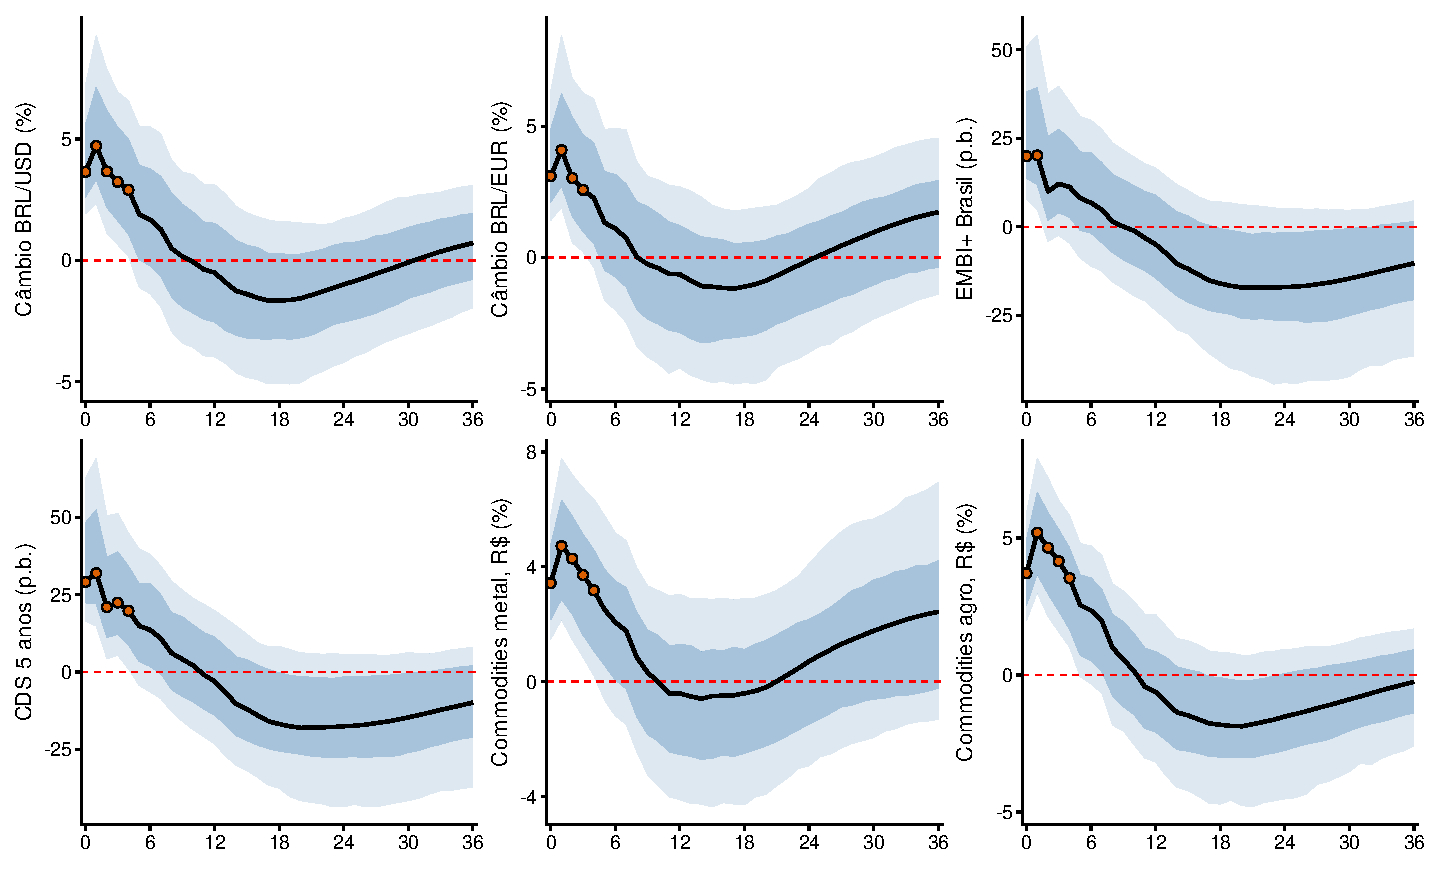
\includegraphics[scale=0.7]{fig_cambio_risco.pdf}
\caption{\textbf{Câmbio e risco soberano}\\{Câmbio em nível de BRL por unidade de moeda estrangeira, convertido para variação percentual pela média amostral, de modo que um valor positivo é depreciação do real. EMBI convertido de pontos percentuais para pontos-base. Os dois últimos painéis são índices de commodities do Banco Central denominados em reais. Pontos laranja marcam os horizontes em que a banda de 90\% exclui zero.}}
%\footnotesize{Source: Own elaboration, based on data from Central Bank.}
\label{fig:cambio}
\end{center} 
\end{figure}

A direção contraria a previsão de manual, segundo a qual o diferencial de juros deveria apreciar a moeda. Ela é compatível, no entanto, com um regime em que a trajetória da dívida pública é a restrição que aperta: nesse cenário, o aumento da taxa de juros piora a dinâmica de rolagem da dívida, e câmbio e spread soberano passam a precificar essa deterioração, em vez do carrego cambial. \cite{goncalves2025} testam essa hipótese para o Brasil com dados diários e a rejeitam, encontrando apreciação cambial de $3,\!4\%$ a $5,\!6\%$ por 100 pontos-base e nenhuma resposta do CDS de cinco anos. A estimativa mensal obtida aqui vai na direção oposta nas duas dimensões, câmbio e risco soberano, uma divergência que discutimos na Seção 5 e que atribuímos, ao menos em parte, à diferença de frequência e de estratégia de identificação entre os dois desenhos. \cite{BEKAERT2013771} documentam, para um conjunto amplo de países, o elo entre política monetária e precificação de risco que a resposta conjunta do EMBI$+$ e do CDS aqui corrobora.



%\begin{figure}[H]
%\caption{Câmbio e risco soberano}
%\label{fig:cambio}
%\centering
%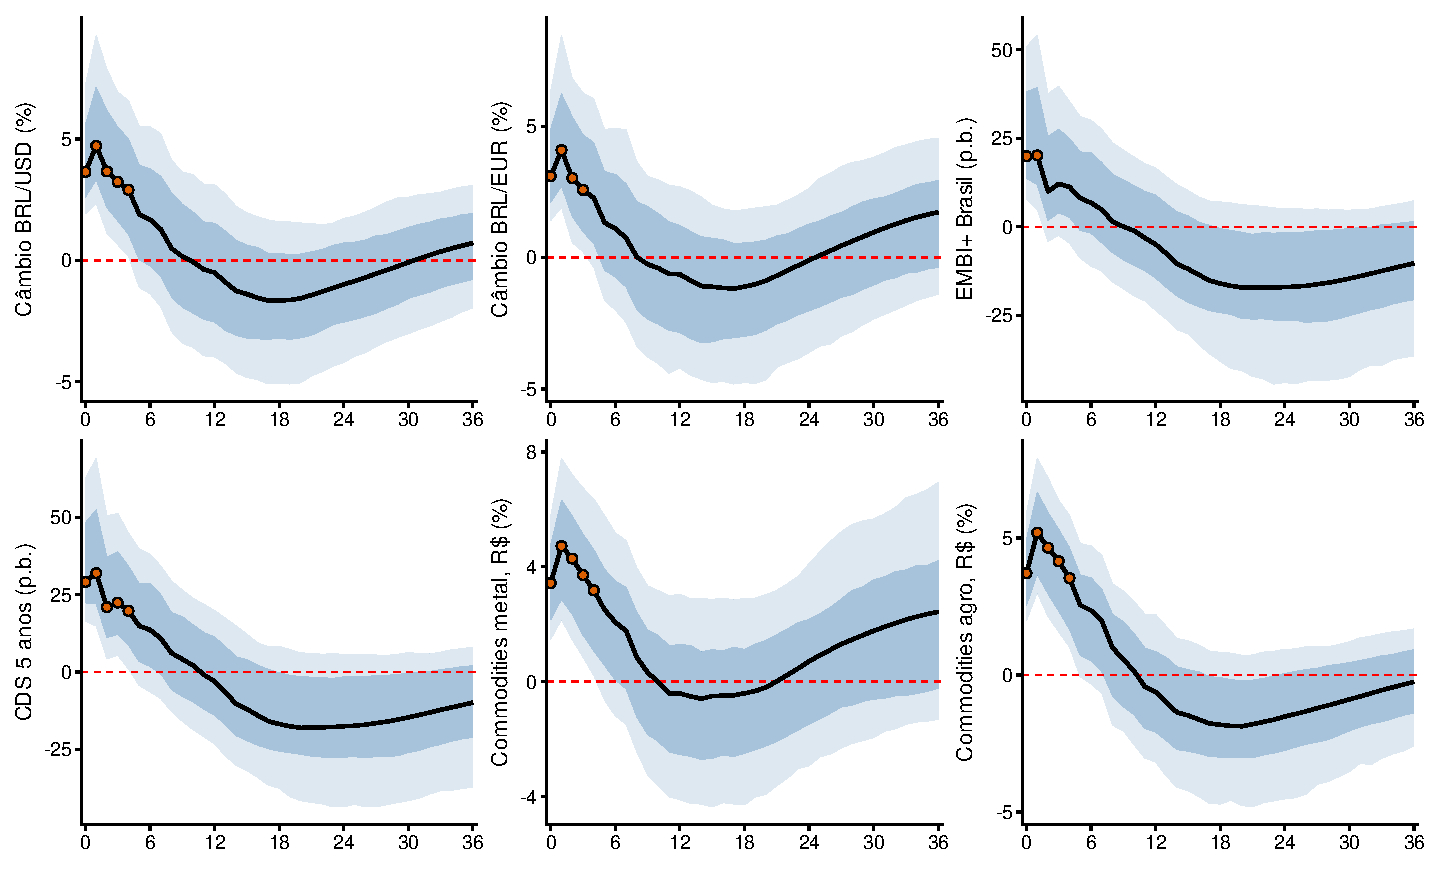
\includegraphics[width=\textwidth]{fig_cambio_risco.pdf}
%\nota{Câmbio em nível de BRL por unidade de moeda estrangeira, convertido para variação percentual pela média amostral, de modo que um valor positivo é depreciação do real. EMBI convertido de pontos percentuais para pontos-base. Os dois últimos painéis são índices de commodities do Banco Central denominados em reais. Pontos laranja marcam os horizontes em que a banda de 90\% exclui zero.}
%\end{figure}

A dinâmica de médio prazo reforça a leitura de um mecanismo comum. O EMBI+ e o CDS revertem de sinal em torno de $h = 10$ e $h = 11$, respectivamente, e permanecem negativos, na banda de $68\%$, entre $h = 18$ e $h  \approx 32$, com mínimos de $-17,\!2$ pontos-base em $h = 22$ e de $-18,\!0$ pontos-base em $h = 20$,  praticamente os mesmos horizontes em que a curva de juros se torna negativa (Seção 4.1), o que sugere o mesmo prêmio revertendo de forma sincronizada em três mercados distintos. O câmbio, por sua vez, não acompanha essa reversão, apenas cobrindo na banda de $68\%$ $h = 0$ a $h = 5$, e a partir de $h = 10$ a estimativa pontual reverte de sinal sem que essa reversão se torne estatisticamente significativa em nenhum horizonte. Essa assimetria temporal, risco soberano persistentemente elevado por mais tempo que o câmbio permanece significativamente depreciado, sugere que o repasse do prêmio de risco ao câmbio é mais rápido de se dissipar do que o próprio aumento da percepção de risco.

%A direção contraria a previsão de manual, na qual o diferencial de juros aprecia a moeda. Ela é a previsão de um regime em que a trajetória da dívida é a restrição que aperta. Nesse cenário, o aumento da taxa piora a dinâmica de rolagem, e câmbio e spread precificam essa deterioração em vez do carrego. \cite{goncalves2025} enunciam essa hipótese para o Brasil e a rejeitam com dados diários, encontrando apreciação de $3{,}4\%$ a $5{,}6\%$ por 100 pontos-base e nenhuma resposta do CDS de 5 anos. A estimativa mensal aqui vai na direção oposta nas duas dimensões. \cite{BEKAERT2013771} documentam o elo entre política monetária e precificação de risco que a resposta do EMBI e do CDS validam.


%Os dois últimos painéis da \autoref{fig:cambio} mostram o mesmo canal por outra via. O índice de commodities metálicas do Banco Central sobe $3{,}43\%$ no impacto e segue significativo até $h = 4$.

%O EMBI e o CDS revertem no médio prazo, na banda de 68\%. Os dois cruzam zero em $h = 10$ e $h = 11$ e ficam negativos de $h = 18$ a $h = 32$ no EMBI e de $h = 18$ a $h = 31$ no CDS, com mínimos de $-17{,}2$ pontos-base em $h = 22$ e de $-18{,}0$ pontos-base em $h = 20$. São os mesmos horizontes em que a curva de juros se torna negativa, e é o mesmo prêmio revertendo em dois mercados com o mesmo compasso. O câmbio não acompanha, sua banda de 68\% cobre apenas $h = 0$ a $h = 5$, e a reversão da estimativa pontual a partir de $h = 10$ não separa de zero em nível algum.

\subsection{Atividade e mercado de trabalho}

A demanda cai no impacto, atinge o vale no décimo primeiro mês e chega ao mercado de trabalho dois anos depois. As três etapas aparecem em níveis de evidência decrescentes, e a seção as separa.

\begin{figure}[H]
\begin{center}
    
\includegraphics[scale=0.7]{fig_atividade.pdf}
\caption{\textbf{Atividade e horas trabalhadas}\\{Índices de quantum e de vendas em nível, convertidos para variação percentual pela média amostral. A utilização da capacidade instalada já está em pontos percentuais. Pontos laranja marcam os horizontes em que a banda de 90\% exclui zero. As seis séries setoriais atingem o vale entre $h = 11$ e $h = 12$, dentro de faixas em que a banda de 68\% exclui zero. O IBC-Br, primeiro painel, acompanha na estimativa pontual e só separa de zero no impacto.}}
%\footnotesize{Source: Own elaboration, based on data from Central Bank.}
\label{fig:atividade}
\end{center} 
\end{figure}

No impacto, a indústria de transformação cai $1{,}37\%$, os bens de consumo duráveis caem $4{,}67\%$, os bens de capital caem $2{,}78\%$, as vendas no varejo caem $1{,}06\%$ e as horas trabalhadas na indústria caem $1{,}08\%$. As cinco respostas excluem zero na banda de 90\%. Na banda de 68\% entram o IBC-Br, com $-0{,}40\%$, e as vendas de serviços, com $-0{,}47\%$, o que estende a queda ao agregado mensal e aos serviços.




%\begin{figure}[H]
%\caption{Atividade e horas trabalhadas}
%\label{fig:atividade}
%\centering
%
\includegraphics[width=\textwidth]{fig_atividade.pdf}
%\nota{Índices de quantum e de vendas em nível, convertidos para variação percentual pela média amostral. A utilização da capacidade instalada já está em pontos percentuais. Pontos laranja marcam os horizontes em que a banda de 90\% exclui zero. As seis séries setoriais atingem o vale entre $h = 11$ e $h = 12$, dentro de faixas em que a banda de 68\% exclui zero. O IBC-Br, primeiro painel, acompanha na estimativa pontual e só separa de zero no impacto.}
%\end{figure}

O fundo cai em $h = 11$ e $h = 12$, na defasagem convencional de transmissão para atividade, e alcança de 1,5 a 2 vezes a queda de impacto. Três séries chegam à banda de 90\%: os bens de capital caem $4{,}93\%$ em $h = 12$, as vendas no varejo caem $1{,}22\%$ em $h = 11$ e a utilização da capacidade instalada cai $0{,}39$ ponto percentual em $h = 11$. As outras três séries setoriais atingem o fundo no mesmo horizonte com banda de 68\%: a indústria de transformação cai $2{,}32\%$, os bens duráveis caem $6{,}71\%$ e as horas trabalhadas caem $1{,}37\%$, todas em $h = 11$, dentro de faixas de 68\% que começam em $h = 8$ e terminam em $h = 16$ na primeira e em $h = 15$ nas outras duas. O agregado mensal não sustenta a afirmação: o IBC-Br acompanha na estimativa pontual, com mínimo de $0{,}50\%$ de queda em $h = 11$, e o impacto é seu único horizonte com banda de 68\%. O vale de transmissão está nas séries setoriais, não no índice agregado.

O mercado de trabalho responde dois anos depois, na banda de 68\% e em nenhum horizonte a 90\%. A taxa de desemprego sobe a partir de $h = 27$ e alcança $+0{,}33$ ponto percentual em $h = 35$. A população ocupada cai a partir de $h = 36$ e chega a $-0{,}69\%$ em $h = 39$. As vendas de serviços voltam à banda de 68\% de $h = 26$ a $h = 38$, com $-1{,}22\%$ em $h = 31$. A defasagem entre a queda da produção no impacto e a resposta do emprego dois anos depois é compatível com o custo de ajuste do fator trabalho. Contra a previsão, a população ocupada sobe no impacto com banda de 68\%, em $+0{,}10\%$.

\subsection{Crédito}

O crédito expande no impacto em três setores e contrai em todos os sete recortes no médio prazo. A expansão de impacto é o único movimento do bloco que alcança a banda de 90\%: o crédito ao setor agropecuário sobe $1{,}01\%$ e permanece significativo até $h = 3$, e o crédito ao setor de transporte sobe $0{,}75\%$ até $h = 1$. Na banda de 68\% entra a indústria, com $+0{,}19\%$, e na direção contrária a construção, com $-0{,}32\%$.



%\begin{figure}[H]
%\caption{Crédito}
%\label{fig:credito}
%\centering
%
\includegraphics[width=\textwidth]{fig_credito.pdf}
%\nota{Saldos de crédito em log-nível, de modo que a resposta está em log-pontos multiplicados por 100, aproximadamente variação percentual. Pontos laranja marcam os horizontes em que a banda de 90\% exclui zero. Só o agropecuário e o transporte têm horizonte significativo a 90\%, e ambos no impacto. Os sete painéis mostram a contração de médio prazo, que exclui zero na banda de 68\% em todos eles.}
%\end{figure}

A leitura da expansão inicial é que as firmas sacam linhas de crédito já aprovadas para financiar capital de giro quando o fluxo de caixa aperta, e que o corte setorial mostra a expansão onde o ciclo de giro é mais pesado. \cite{Cooley} obtêm, em equilíbrio geral com firmas heterogêneas em patrimônio líquido e porte, que a estrutura financeira da firma condiciona sua resposta ao choque monetário. A heterogeneidade setorial documentada aqui é uma margem distinta, a segmentação entre crédito direcionado e livre. A construção, que contrai desde o impacto, é o setor de ciclo mais longo e mais sensível à taxa longa.

A contração agregada existe na banda de 68\% e é ordenada. Os sete recortes ficam negativos a partir de um ponto entre $h = 15$ e $h = 22$, e os fundos são de $-2{,}44\%$ em $h = 29$ na construção, $-2{,}19\%$ em $h = 26$ no comércio, $-1{,}97\%$ em $h = 24$ no transporte, $-1{,}63\%$ em $h = 25$ na indústria, $-1{,}47\%$ em $h = 25$ no agropecuário, $-1{,}23\%$ em $h = 29$ no saldo total e $-0{,}94\%$ em $h = 32$ na pessoa física. Os três setores que expandem no impacto são os mesmos que contraem depois, e a distância entre os dois movimentos é de cerca de dois anos. Nenhuma dessas respostas separa de zero na banda de 90\%.

\begin{figure}[H]
\begin{center}
    
\includegraphics[scale=0.7]{fig_credito.pdf}
\caption{\textbf{Crédito}\\{Saldos de crédito em log-nível, de modo que a resposta está em log-pontos multiplicados por 100, aproximadamente variação percentual. Pontos laranja marcam os horizontes em que a banda de 90\% exclui zero. Só o agropecuário e o transporte têm horizonte significativo a 90\%, e ambos no impacto. Os sete painéis mostram a contração de médio prazo, que exclui zero na banda de 68\% em todos eles.}}
%\footnotesize{Source: Own elaboration, based on data from Central Bank.}
\label{fig:credito}
\end{center} 
\end{figure}

Os dois spreads do indicador de custo do crédito comprimem no impacto e alargam depois, com pico de $+0{,}134$ ponto percentual em $h = 11$ na pessoa física e de $+0{,}069$ em $h = 14$ na pessoa jurídica, ambos com banda de 68\%. A compressão inicial é propriedade da medida, porque o indicador é a taxa média da carteira em estoque e reprecifica devagar. O alargamento tardio é compatível com o acelerador financeiro de \cite{BERNANKE19991341}, chegando na defasagem em que o estoque já reprecificou.

\subsection{Preços}

Toda resposta de preço que exclui zero a 90\% é positiva, e nenhuma medida de inflação produz resposta negativa significativa em horizonte algum. O índice de preços ao produtor é significativo de $h = 0$ a $h = 4$, com pico de $+0{,}88$ ponto percentual em $h = 1$. O IGP-M é significativo de $h = 1$ a 4, com pico de $+0{,}41$ em $h = 2$. O IPCA cheio é significativo apenas em $h = 5$, com $+0{,}18$. O núcleo por exclusão EX0 é significativo em $h = 2$ e de $h = 4$ a 8, com pico de $+0{,}13$ em $h = 5$, e o núcleo de médias aparadas em $h = 4$, 5 e 7, com pico de $+0{,}09$.


%\begin{figure}[H]
%\caption{Preços}
%\label{fig:precos}
%\centering
%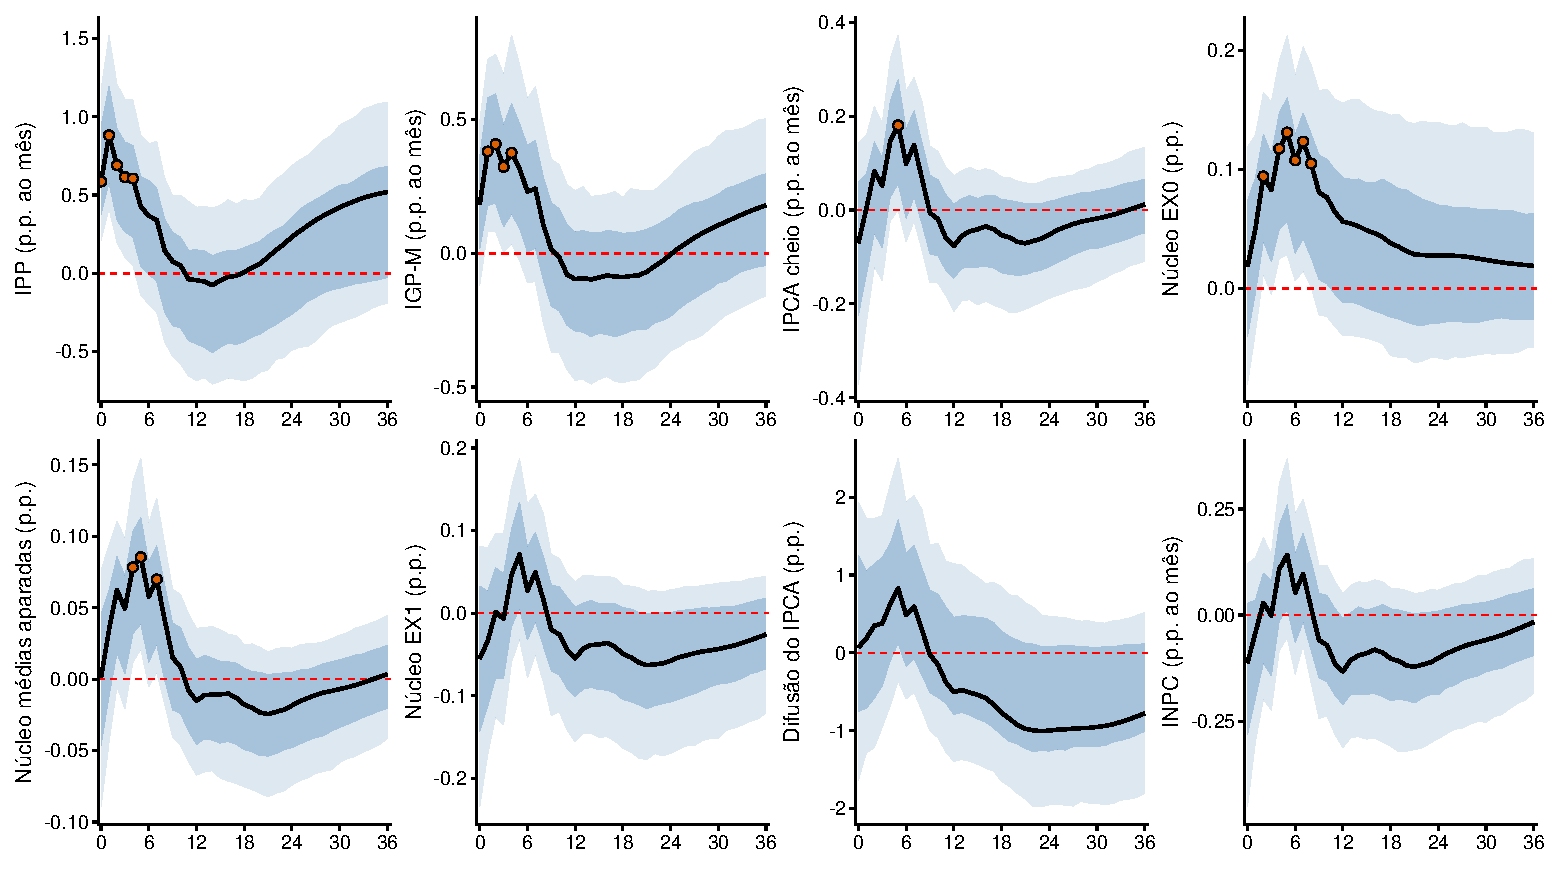
\includegraphics[width=\textwidth]{fig_precos.pdf}
%\nota{As séries de inflação entram no painel como taxa mensal, de modo que a resposta está em pontos percentuais da taxa mensal, cuja média amostral no IPCA é de $0{,}47$. Índice de difusão em pontos percentuais da proporção de itens com alta. Pontos laranja marcam os horizontes em que a banda de 90\% exclui zero. Os três últimos painéis não têm nenhum horizonte significativo a 90\%: o mínimo da estimativa pontual é de $-0{,}06$ em $h = 21$ no núcleo EX1, de $-1{,}01$ em $h = 23$ no índice de difusão e de $-0{,}13$ em $h = 12$ no INPC.}
%\end{figure}

A ordenação temporal entre as medidas é o que a figura adiciona ao diagnóstico. O índice de preços ao produtor responde já no impacto, na mesma janela em que o câmbio se deprecia com banda de 90\%, e as medidas ao consumidor respondem depois, entre o quarto e o oitavo mês. A sequência é compatível com repasse cambial por custo, com origem no canal da \autoref{sec:cambio}. Em uma economia cuja moeda se deprecia $3{,}64\%$ no impacto de um aperto, o sinal positivo de curto prazo nos preços tem uma leitura econômica.

\cite{jarocinski2020} tratam o \textit{price puzzle} isolando o choque de política com um filtro de sinal que torna a desinflação americana mais pronunciada. Embora essa técnica opere como a terceira camada do instrumento utilizado aqui, o sinal positivo nos preços sobrevive à estimativa.

A desinflação que a teoria prevê existe no painel e é a evidência mais fraca de toda a seção. O núcleo por exclusão EX1 é negativo de $h = 9$ a $h = 45$, com mínimo de $-0{,}063$ ponto percentual em $h = 21$, e sua banda de 68\% exclui zero em exatamente dois horizontes, $h = 21$ e $h = 22$. É a única medida de preço com veredito de coerência forte na verificação de janelas teóricas. O índice de difusão acompanha na estimativa pontual, com a proporção de itens em alta caindo de $h = 9$ até o mínimo de $-1{,}01$ ponto percentual em $h = 23$.

\begin{figure}[H]
\begin{center}
    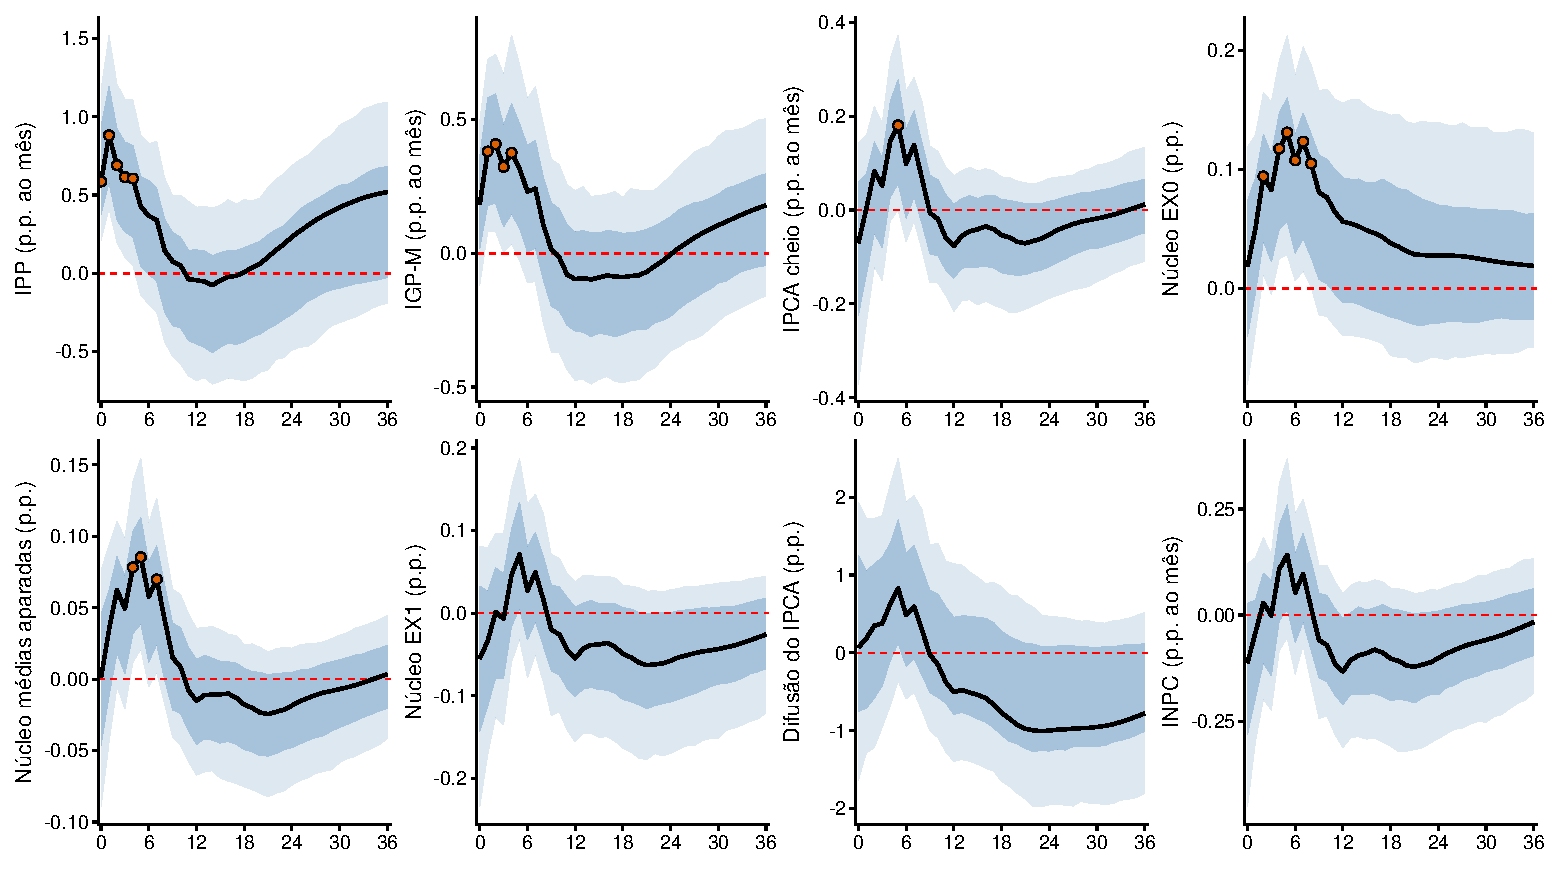
\includegraphics[scale=0.7]{fig_precos.pdf}
\caption{\textbf{Preços}\\{As séries de inflação entram no painel como taxa mensal, de modo que a resposta está em pontos percentuais da taxa mensal, cuja média amostral no IPCA é de $0{,}47$. Índice de difusão em pontos percentuais da proporção de itens com alta. Pontos laranja marcam os horizontes em que a banda de 90\% exclui zero. Os três últimos painéis não têm nenhum horizonte significativo a 90\%: o mínimo da estimativa pontual é de $-0{,}06$ em $h = 21$ no núcleo EX1, de $-1{,}01$ em $h = 23$ no índice de difusão e de $-0{,}13$ em $h = 12$ no INPC.}}
%\footnotesize{Source: Own elaboration, based on data from Central Bank.}
\label{fig:precos}
\end{center} 
\end{figure}

O núcleo por exclusão EX0 é o único veredito de incoerência do painel na verificação de janelas teóricas. Ele é positivo em todos os horizontes entre $h = 12$ e $h = 48$, e não retorna a território negativo no médio prazo, ao contrário do IPCA cheio, do núcleo de médias aparadas e do INPC. 

\subsection{Ações}

Nenhum dos oito índices da B3 separa de zero a 90\% em qualquer horizonte. O bloco não sustenta uma afirmação de significância estatística, e o que segue está todo na banda de 68\% ou na estimativa pontual.


%\begin{figure}[H]
%\caption{Índices de ações}
%\label{fig:acoes}
%\centering
%
\includegraphics[width=\textwidth]{fig_acoes.pdf}
%\nota{Os índices da B3 entram no painel como retorno mensal e a resposta é acumulada para recuperar o nível de preço, em pontos percentuais. Bandas de 68\% e 90\%. A ausência de marcadores laranja é o resultado: nenhum dos oito índices exclui zero a 90\% em nenhum dos 49 horizontes estimados. A banda de 68\% positiva a partir de $h \approx 14$ no Ibovespa e no índice financeiro é deriva de acúmulo, discutida no texto.}
%\end{figure}

Os oito índices caem no impacto, entre $-0{,}31\%$ e $-2{,}89\%$, e a queda se aprofunda em $h = 1$. Quatro deles separam de zero na banda de 68\% já no impacto, e em $h = 1$ são sete dos oito, todos negativos: IMOB $-5{,}49\%$, SMLL $-5{,}36\%$, IDIV $-3{,}57\%$, MLCX $-3{,}29\%$, IFNC $-3{,}27\%$, Ibovespa $-3{,}11\%$ e IFIX $-2{,}70\%$. O único ausente é o IMAT, índice de materiais básicos, cujos componentes são exportadores amortecidos pela depreciação da mesma janela. A ordenação segue a previsão de canal financeiro, com incorporadoras imobiliárias e \textit{small caps} caindo mais que o índice amplo. O IFIX é o único índice negativo em todos os 49 horizontes, com banda de 68\% de $h = 0$ a $h = 8$, e fundos de renda imobiliária de fato precificam como renda fixa longa.

\begin{figure}[H]
\begin{center}
    
\includegraphics[scale=0.7]{fig_acoes.pdf}
\caption{\textbf{Índices de ações}\\{Os índices da B3 entram no painel como retorno mensal e a resposta é acumulada para recuperar o nível de preço, em pontos percentuais. Bandas de 68\% e 90\%. A ausência de marcadores laranja é o resultado: nenhum dos oito índices exclui zero a 90\% em nenhum dos 49 horizontes estimados. A banda de 68\% positiva a partir de $h \approx 14$ no Ibovespa e no índice financeiro é deriva de acúmulo, discutida no texto.}}
%\footnotesize{Source: Own elaboration, based on data from Central Bank.}
\label{fig:acoes}
\end{center} 
\end{figure}

O Ibovespa cai $1{,}67\%$ no impacto, e a banda de 90\% vai de $-7{,}77\%$ a $+1{,}76\%$. A magnitude está dentro da faixa que os estudos de evento em dias de Copom encontram para o Brasil, de 1\% a 2\% por 100 pontos-base.



%---------------
\section{Concluding remarks}
%%---------------
Este artigo documenta um fato estilizado que contraria o mecanismo convencional da paridade descoberta de juros: em uma economia emergente com histórico de fragilidade fiscal, um aperto monetário pode elevar o prêmio de risco soberano a ponto de depreciar, em vez de apreciar, a moeda doméstica. Usando um modelo de fatores dinâmicos estruturais identificado por instrumento externo sobre um painel de mais de 100 séries macroeconômicas e financeiras brasileiras, mostramos que um choque contracionista de 50 pontos-base deprecia o real em $3,\!64\%$ no impacto, ao mesmo tempo em que o EMBI+ e o CDS soberano de cinco anos se abrem, uma resposta conjunta incompatível com o canal tradicional do diferencial de juros, mas consistente com um regime em que o aumento da taxa de juros piora a percepção sobre a sustentabilidade da dívida.

A curva de juros reforça essa interpretação. O repasse do choque cresce com a maturidade até cinco anos, superando a amplificação documentada para economias desenvolvidas. No médio prazo, as taxas de juros e as medidas de risco soberano exibem uma dinâmica de reversão altamente sincronizada, ao passo que o câmbio perde significância estatística bem antes dessa reversão, sugerindo que o aumento do prêmio de risco é mais persistente do que seu repasse à taxa de câmbio.

%A curva de juros reforça essa leitura. O repasse do choque cresce com a maturidade até cinco anos, superando a amplificação que desenhos comparáveis encontram em economias desenvolvidas, e reverte no médio prazo em estreita sincronia com o câmbio e o prêmio de risco soberano, os cinco vértices, o EMBI+ e o CDS revertem de sinal em janelas próximas, entre o décimo e o vigésimo quarto mês. O câmbio, no entanto, não acompanha essa reversão: sua resposta perde significância estatística já a partir do quinto mês, sugerindo que o efeito sobre o risco soberano é mais persistente do que seu repasse ao câmbio.

Os demais resultados sugerem que esse canal de prêmio de risco opera em paralelo aos canais tradicionais de transmissão da política monetária. A atividade econômica desacelera, o mercado de trabalho responde com defasagem, o crédito inicialmente se expande antes de contrair de forma mais disseminada, e a inflação apresenta evidências de repasse cambial no curto prazo, o mercado acionário é a exceção, sem resposta estatisticamente significativa em nenhum dos oito índices setoriais analisados. Em conjunto, esses resultados indicam que o aumento do prêmio de risco soberano não substitui os canais convencionais de transmissão, mas passa a coexistir com eles em contextos de fragilidade fiscal como o brasileiro.

Nossos resultados contrastam com evidências recentes para o Brasil obtidas por identificação via heterocedasticidade em frequência diária, que rejeitam a hipótese de dominância fiscal \citep[]{goncalves2025}. Longe de serem contraditórias, essas evidências sugerem que a importância do canal de prêmio de risco pode depender da frequência dos dados e da estratégia de identificação utilizada, um choque identificado por surpresas de mercado em janela diária pode capturar uma dinâmica de curto prazo distinta da resposta mensal, mais persistente, que documentamos aqui. Reconciliar essas duas evidências é uma questão em aberto que deixamos para pesquisa futura, possivelmente por meio de um desenho que combine ambas as frequências de identificação sobre a mesma base de dados.

Do ponto de vista de política econômica, nossos resultados indicam que, em economias emergentes sujeitas a fragilidades fiscais, a eficácia do canal cambial da política monetária não deve ser assumida automaticamente a partir do mecanismo convencional da paridade descoberta da taxa de juros. Nesses contextos, a credibilidade fiscal, e não apenas a magnitude do choque monetário, passa a condicionar a direção da resposta cambial. Mais amplamente, nossos resultados sugerem que a transmissão da política monetária deve ser compreendida como o resultado da interação entre política monetária e percepção de risco soberano, e não apenas como consequência do diferencial de juros. Essa perspectiva amplia a interpretação tradicional do canal cambial e, no caso brasileiro, oferece uma explicação alternativa para episódios em que aumentos da taxa básica de juros são acompanhados por depreciação cambial, um padrão que pode ser relevante para outras economias emergentes sujeitas a preocupações semelhantes de sustentabilidade fiscal.

%\section*{Funding}
%Jo\~ao F. Caldeira gratefully acknowledges support provided by CNPq under grant 309448/2022-0.

%%---------------
%% Bibliografia
%%---------------
%\section*{References}
\bibliographystyle{authordate3} % bibliography style
\bibliography{references} % References file

\section*{Appendix}\label{anexo-A}

\begin{ThreePartTable}
\begin{TableNotes}
\footnotesize
\item[*] Código de transformação com que a série entra na extração de fatores e é recuperada em unidades econômicas na função de impulso-resposta. 1 = nível. 2 = retorno mensal, com a função de impulso-resposta acumulada para recuperar a resposta de nível de preço. 4 = log-nível. Os índices de mercado da B3 entram como retorno mensal. Os volumes nominais (base monetária, agregados, crédito, PIB e recolhimentos compulsórios) entram em logaritmo. As séries com sazonalidade detectada são ajustadas por X-13ARIMA-SEATS \cite{sax2018seasonal}. Todas as séries são padronizadas pelo desvio padrão da primeira diferença \cite{barigozzi2016non} antes da extração de fatores. As séries em nível não são diferenciadas, a não-estacionariedade é acomodada pela padronização.
\end{TableNotes}

\footnotesize
\setlength{\tabcolsep}{4pt}
\begin{longtable}{@{}p{5.2cm} l l c@{}}
\caption{Lista de Variáveis Utilizadas}\label{tab:lista_variaveis} \\
\toprule
\textbf{Variável} & \textbf{Fonte} & \textbf{Grupo} & \textbf{Código} \\
\midrule
\endfirsthead

\toprule
\textbf{Variável} & \textbf{Fonte} & \textbf{Grupo} & \textbf{Código} \\
\midrule
\endhead



\bottomrule
\insertTableNotes
\endlastfoot

Câmbio USD/BRL & Yahoo Finance & Câmbio & 1 \\
Câmbio EUR/BRL & Yahoo Finance & Câmbio & 1 \\
Câmbio CNY/BRL & Yahoo Finance & Câmbio & 1 \\
Câmbio ARS/BRL & Yahoo Finance & Câmbio & 1 \\
Câmbio INR/BRL & Yahoo Finance & Câmbio & 1 \\
Selic (meta acumulada) & BCB (4189) & Juros e curva & 1 \\
CDI acumulado & BCB (4392) & Juros e curva & 1 \\
DI 3 meses & Svensson/B3 & Juros e curva & 1 \\
DI 6 meses & Svensson/B3 & Juros e curva & 1 \\
DI 1 ano & Svensson/B3 & Juros e curva & 1 \\
DI 2 anos & Svensson/B3 & Juros e curva & 1 \\
DI 5 anos & Svensson/B3 & Juros e curva & 1 \\
DI 10 anos & Svensson/B3 & Juros e curva & 1 \\
Base monetária & BCB (1788) & Agregados monetários & 4 \\
Meios de pagamento & BCB (27789) & Agregados monetários & 4 \\
Depósitos à vista & BCB (27790) & Agregados monetários & 4 \\
Depósitos de poupança & BCB (1835) & Agregados monetários & 4 \\
M1 & BCB (27791) & Agregados monetários & 4 \\
M2 & BCB (27810) & Agregados monetários & 4 \\
M3 & BCB (27813) & Agregados monetários & 4 \\
Crédito agropecuário & BCB (22027) & Crédito & 4 \\
Crédito indústria & BCB (22043) & Crédito & 4 \\
Crédito construção & BCB (22030) & Crédito & 4 \\
Crédito comércio & BCB (22036) & Crédito & 4 \\
Crédito transporte & BCB (22037) & Crédito & 4 \\
Crédito pessoa física & BCB (22050) & Crédito & 4 \\
Spread ICC pessoa jurídica & BCB (27444) & Crédito & 1 \\
Spread ICC pessoa física & BCB (27445) & Crédito & 1 \\
Saldo de crédito total & BCB (20542) & Crédito & 4 \\
Recolhimentos compulsórios & BCB (17633) & Crédito & 4 \\
Consumo de gasolina & BCB (1393) & Atividade econômica & 1 \\
Consumo de GLP & BCB (1394) & Atividade econômica & 1 \\
Consumo de óleo combustível & BCB (1395) & Atividade econômica & 1 \\
Consumo de óleo diesel & BCB (1396) & Atividade econômica & 1 \\
Consumo de demais derivados & BCB (1397) & Atividade econômica & 1 \\
Consumo de álcool & BCB (1401) & Atividade econômica & 1 \\
Utilização da capacidade instalada (CNI) & BCB (28554) & Atividade econômica & 1 \\
Vendas no varejo & BCB (1455) & Atividade econômica & 1 \\
Vendas de serviços & BCB (23982) & Atividade econômica & 1 \\
Produção de automóveis & BCB (7384) & Atividade econômica & 1 \\
Produção de veículos leves & BCB (7385) & Atividade econômica & 1 \\
Produção de caminhões & BCB (7386) & Atividade econômica & 1 \\
Produção de ônibus & BCB (7387) & Atividade econômica & 1 \\
Produção de bens de consumo & BCB (21865) & Atividade econômica & 1 \\
Produção de bens duráveis & BCB (21866) & Atividade econômica & 1 \\
Produção de bens não duráveis & BCB (21867) & Atividade econômica & 1 \\
Produção de bens de capital & BCB (21863) & Atividade econômica & 1 \\
Produção da indústria de transformação & BCB (21862) & Atividade econômica & 1 \\
Produção da indústria extrativa & BCB (21861) & Atividade econômica & 1 \\
Utilização da capacidade instalada (FGV) & BCB (24352) & Atividade econômica & 1 \\
Consumo de energia comercial & BCB (1402) & Atividade econômica & 1 \\
Consumo de energia residencial & BCB (1403) & Atividade econômica & 1 \\
Consumo de energia industrial & BCB (1404) & Atividade econômica & 1 \\
Consumo de energia outros & BCB (1405) & Atividade econômica & 1 \\
PIB acumulado no ano & BCB (4381) & Atividade econômica & 4 \\
IBC-Br & BCB (24364) & Atividade econômica & 1 \\
Índice de confiança do consumidor & BCB (4393) & Atividade econômica & 1 \\
Índice de confiança de serviços & BCB (17660) & Atividade econômica & 1 \\
Emprego formal Sudeste & BCB (13901) & Mercado de trabalho & 1 \\
Emprego formal Sul & BCB (13564) & Mercado de trabalho & 1 \\
Emprego formal Nordeste & BCB (13941) & Mercado de trabalho & 1 \\
Emprego formal Norte & BCB (28152) & Mercado de trabalho & 1 \\
Emprego formal Centro-Oeste & BCB (21991) & Mercado de trabalho & 1 \\
Salário mínimo & BCB (1619) & Mercado de trabalho & 1 \\
População na força de trabalho & BCB (24378) & Mercado de trabalho & 1 \\
População ocupada & BCB (28543) & Mercado de trabalho & 1 \\
Taxa de desemprego & BCB (24369) & Mercado de trabalho & 1 \\
Horas trabalhadas na indústria & BCB (28556) & Mercado de trabalho & 1 \\
Tempo de procura: até 1 mês & IBGE/SIDRA (1616) & Mercado de trabalho & 1 \\
Tempo de procura: 1 mês a 1 ano & IBGE/SIDRA (1616) & Mercado de trabalho & 1 \\
Tempo de procura: 1 a 2 anos & IBGE/SIDRA (1616) & Mercado de trabalho & 1 \\
Tempo de procura: 2 anos ou mais & IBGE/SIDRA (1616) & Mercado de trabalho & 1 \\
IPCA & BCB (433) & Inflação & 1 \\
IPCA índice de difusão & BCB (21379) & Inflação & 1 \\
IPCA núcleo EX0 & BCB (29677) & Inflação & 1 \\
IPCA núcleo EX1 & BCB (29678) & Inflação & 1 \\
IPCA núcleo médias aparadas & BCB (16122) & Inflação & 1 \\
IGP-M & BCB (189) & Inflação & 1 \\
IPC & BCB (191) & Inflação & 1 \\
IPC núcleo & BCB (4467) & Inflação & 1 \\
INCC & BCB (192) & Inflação & 1 \\
INPC & BCB (188) & Inflação & 1 \\
IPP & IPEA (IPP12\_IPPCG12) & Inflação & 1 \\
Índice de commodities agropecuária & BCB (27575) & Commodities & 1 \\
Índice de commodities metal & BCB (27576) & Commodities & 1 \\
Índice de commodities energia & BCB (27577) & Commodities & 1 \\
Ibovespa (retorno mensal) & B3 & Índices de mercado & 2 \\
IDIV (retorno mensal) & B3 & Índices de mercado & 2 \\
IFIX (retorno mensal) & B3 & Índices de mercado & 2 \\
IFNC (retorno mensal) & B3 & Índices de mercado & 2 \\
IMAT (retorno mensal) & B3 & Índices de mercado & 2 \\
IMOB (retorno mensal) & B3 & Índices de mercado & 2 \\
MLCX (retorno mensal) & B3 & Índices de mercado & 2 \\
SMLL (retorno mensal) & B3 & Índices de mercado & 2 \\
EMBI+ Brasil & JP Morgan & Risco e incerteza & 1 \\
CDS soberano 5 anos & Investing.com & Risco e incerteza & 1 \\
MSCI mercados emergentes & Investing.com & Risco e incerteza & 1 \\
VIX & CBOE & Risco e incerteza & 1 \\
EPU Brasil & policyuncertainty.com & Risco e incerteza & 1 \\
EPU Canadá & policyuncertainty.com & Risco e incerteza & 1 \\
EPU Chile & policyuncertainty.com & Risco e incerteza & 1 \\
EPU China & policyuncertainty.com & Risco e incerteza & 1 \\
EPU Alemanha & policyuncertainty.com & Risco e incerteza & 1 \\
EPU Índia & policyuncertainty.com & Risco e incerteza & 1 \\
EPU Rússia & policyuncertainty.com & Risco e incerteza & 1 \\
EPU Estados Unidos & policyuncertainty.com & Risco e incerteza & 1 \\

\end{longtable}
\end{ThreePartTable}





\end{document}
